\documentclass[a4paper,12pt]{article}

\usepackage[top=3cm, bottom=2cm, left=3cm, right=2cm]{geometry}
\usepackage[utf8]{inputenc}
\usepackage[portuguese]{babel}
\usepackage{booktabs}
\usepackage{multirow}
\usepackage{multicol}
\usepackage{graphicx}
\usepackage{longtable}
\usepackage{verbatim}

\usepackage{float}
\floatstyle{ruled}
\newfloat{program}{thp}{lop}
\floatname{program}{Script}

\title{Tecnologias de Base de Dados}

\author{André Fernandes (ei03107) \and Pedro Batista (ext10392)}

\begin{document}

\maketitle

\section{Modelo de classes}

	\begin{figure}[htp]
		\begin{center}
			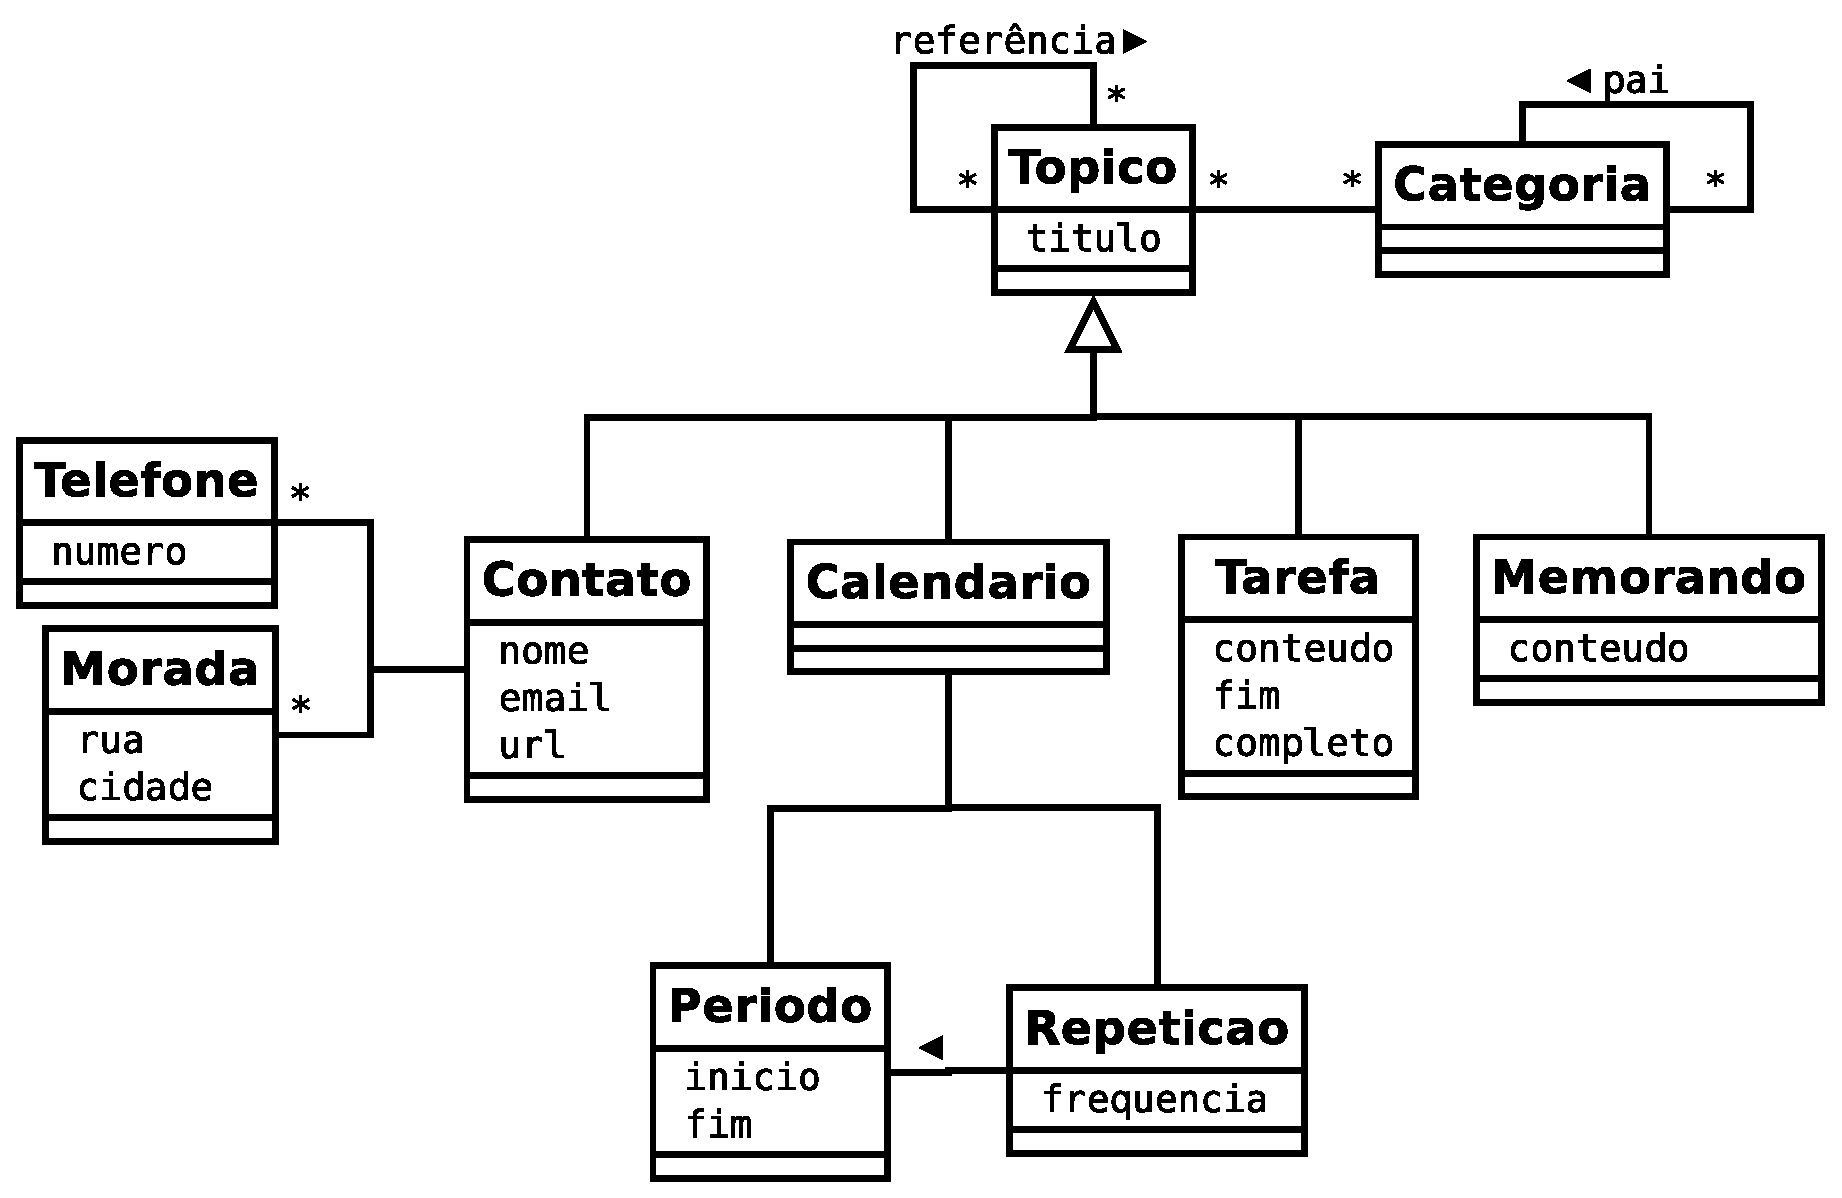
\includegraphics[height=300pt]{uml}
		\end{center}
		\caption{Modelo de classes.}
		\label{fig:uml}
	\end{figure}

\section{Modelo relacional}


\section{Modelo de dados}

	\begin{multicols}{2}
		\begin{tabular}{|c|l|} \hline
		\multirow{4}{*}{TOPICO}
		& titulo VARCHAR(25) \\
		& alteracao DATETIME \\ 
		& categorias S\_CATEGORIA \\
		& referencias S\_TOPICO\\ \hline 
		\end{tabular}
		
		\begin{tabular}{|c|l|} \hline
		\multirow{4}{*}{CONTATO}
		& nome VARCHAR(25) \\
		& telefones S\_TELEFONE \\ 
		& moradas S\_MORADA \\
		& email VARCHAR(100) \\ 
		& url VARCHAR(200) \\ \hline 
		\end{tabular}
		
		\begin{tabular}{|c|l|} \hline
		\multirow{2}{*}{CALENDARIO}
		& p PERIODO \\
		& r REPETICAO \\ \hline 
		\end{tabular}
		
		\begin{tabular}{|c|l|} \hline
		\multirow{3}{*}{TAREFA}
		& fim DATETIME \\
		& completo VARCHAR(1) \\ 
		& conteudo VARCHAR(255) \\ \hline 
		\end{tabular}
		
		\begin{tabular}{|c|l|} \hline
		MEMO & fim DATETIME \\ \hline
		\end{tabular}
		
		\begin{tabular}{|c|l|} \hline
		\multirow{2}{*}{CATEGORIA}
		& nome VARCHAR(25) \\
		& pai REF CATEGORIA \\ \hline 
		\end{tabular}
		
		\begin{tabular}{|c|l|} \hline
		\multirow{2}{*}{REPETICAO}
		& frequencia VARCHAR(7) \\
		& p PERIODO \\ \hline 
		\end{tabular}
		
		\begin{tabular}{|c|l|} \hline
		\multirow{2}{*}{PERIODO}
		& inicio DATETIME \\
		& fim DATETIME \\ \hline 
		\end{tabular}
		
		\begin{tabular}{|c|l|} \hline
		\multirow{2}{*}{MORADA}
		& rua VARCHAR(100) \\
		& cidade VARCHAR(50) \\ \hline 
		\end{tabular}
		
		\begin{tabular}{|c|l|} \hline
		TELEFONE & numero VARCHAR(25) \\ \hline 
		\end{tabular}
		
		\begin{tabular}{|c|l|} \hline
		S\_CATEGORIA & SET(CATEGORIA) \\ \hline
		\end{tabular}
		
		\begin{tabular}{|c|l|} \hline
		S\_TOPICO & SET(REF TOPICO) \\ \hline
		\end{tabular}
		
		\begin{tabular}{|c|l|} \hline
		S\_MORADA & SET(MORADA) \\ \hline
		\end{tabular}
		
		\begin{tabular}{|c|l|} \hline
		S\_TELEFONE & SET(TELEFONE) \\ \hline
		\end{tabular}

	\end{multicols}




\end{document}
